\documentclass{article}
\usepackage{graphicx} % Required for inserting images
\usepackage{lipsum}
\usepackage{amsmath}
\usepackage{amssymb}
\usepackage{xfrac}
\usepackage{caption}
\usepackage{subcaption}


\title{Orbital Geometry Guide}
\author{Sara Pessognelli}
\date{\today}
\begin{document}

\maketitle

\begin{abstract}

\end{abstract}
\newpage

\section*{Coordinate Systems}
\subsection*{ECEF, Polar, \& Latitude-Longitude Coordinates}

\begin{figure}
    \centering
    \begin{subfigure}{.5\textwidth}
      \centering
      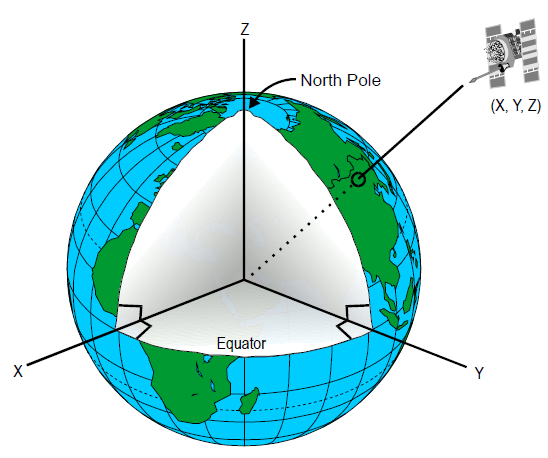
\includegraphics[scale=0.4]{Earth_Centered_Inertial_Coordinate_System}
      \caption{Earth-center, Earth-fixed reference frame (ECEF).}
      \label{fig:sub1}
    \end{subfigure}%
    \begin{subfigure}{.5\textwidth}
      \centering
      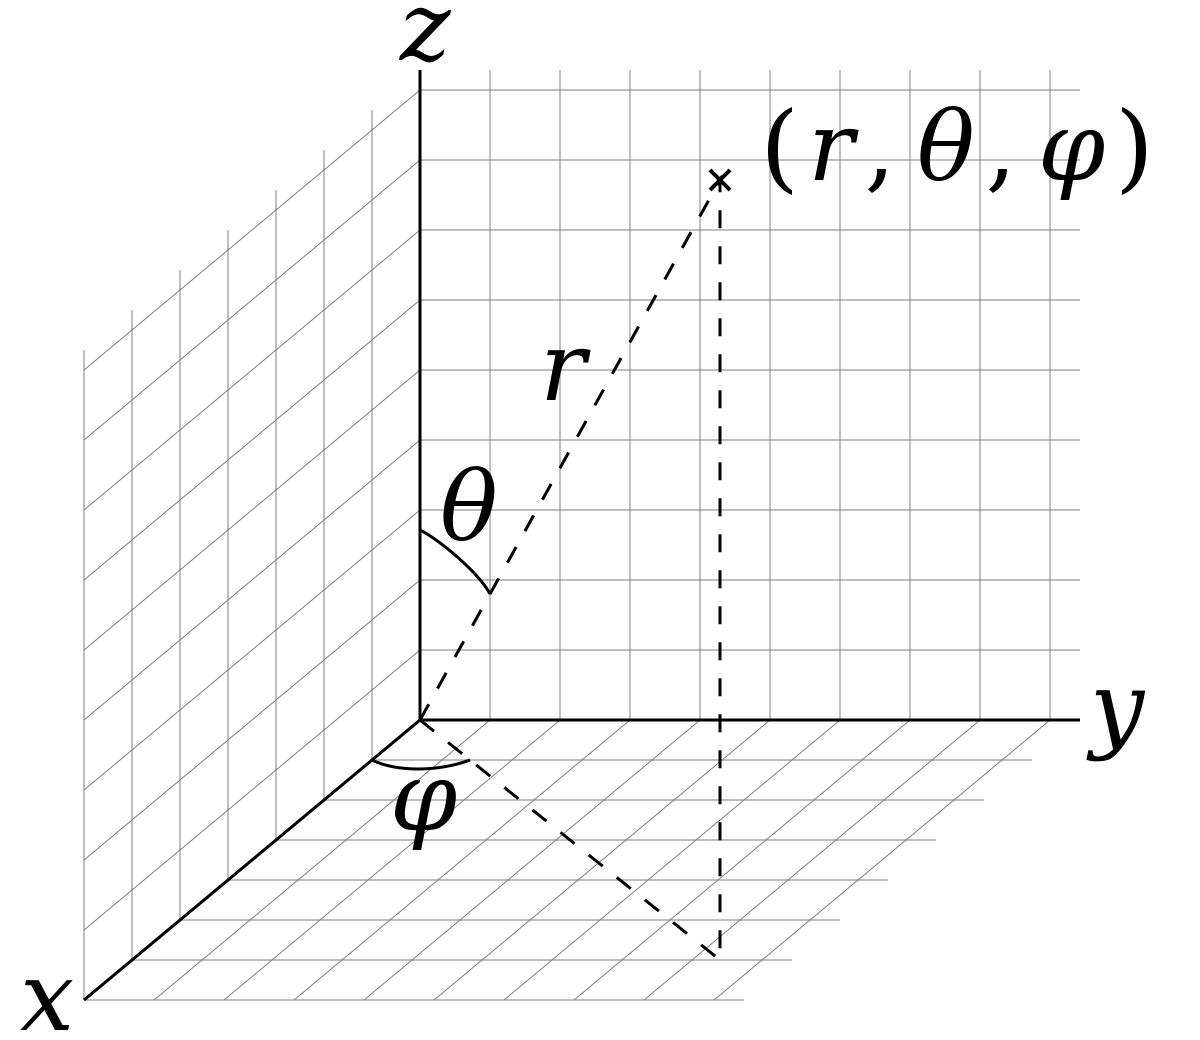
\includegraphics[scale=0.15]{polarSystem.PNG} 
      \caption{Polar ($\theta, \phi$) reference frame.}
      \label{fig:sub2}
    \end{subfigure}
    \caption{Comparison of the ECEF and Polar reference frames.}
    \label{fig:test}
    \end{figure}

In Figure 1 (a) of the \textbf{ECEF} reference frame, the $z^+$-axis is the North Pole, 
$x^+$ passes through the intersection of
the Equator ($0^{\circ}$ latitude) and Prime Meridian ($0 \deg$ longitude), and the $y^+$-axis passes
through the Equator and $90^{\circ}$ longitude arc. \\\\
Figure 1 (b) shows us that in the \textbf{polar} coordinate system, $\theta$ is the angle 
measured down from the $z^+$-axis 
toward the $xy$-plane, and $\phi$ is the angle measured from
the $x^+$-axis, counterclockwise. \\\\
The only difference between the polar coordinate system and the \textbf{latitude-longitude} coordinate 
system is that a point's latitude is measured up from the $xy-$plane towards the $z^+$ axis. In order
to find the \textbf{altitude} we simply take $$\text{Alt} = r - r_e$$, where $r_e$ is the radius of the 
Earth at that point. (Note: the Earth is eliptical, but for the sake of the calculations in this
guide, we will be assuming a spherical Earth with radius $r_e = 6378$ km.)
\\\\
The conversions between these frames is as follows:
\\
\subsubsection*{Polar-to-LLA}
$$\text{Latitude} = \Theta = 90-\theta$$
$$\text{Longitude} = \Phi = \phi$$
\subsubsection*{ECEF-to-LLA (and Polar!)}
$$r = \sqrt{x^2 + y^2 + z^2}$$
$$\text{Alt} = r - r_e$$
$$\theta = \cos^{-1}(\frac{z}{r})$$
$$\text{Latitude} = 90^{\circ} - \cos^{-1}(\frac{z}{r})$$
$$\text{Longitude} = \phi = \tan^{-1}(\frac{y}{x})$$
\subsubsection*{LLA-to-ECEF}
$$x = r\cos(Latitude)\cos(Longitude)$$
$$y = r\cos(Latitude)\sin(Longitude)$$
$$z = r\sin(Latitude)$$
\subsubsection*{Polar-to-ECEF}
$$x = r\sin(\theta)\cos(\phi)$$
$$y = r\sin(\theta)\sin(\phi)$$
$$z = r\cos(\theta)$$

\subsubsection*{Platform-centered Coordinate Systems (PCCS)}
The local coordinate system of the platforms has the \textbf{nadir} vector (that is, the vector 
pointing from the center of the platform to the center of Earth) as the $z^+$-axis. 
The sub-platform point (SPP) is the point at which the nadir line intersects the surface of the Earth.
In the PCCSs, the $x^+$-axis parllel to, and directionally the same, as the northward vector of the
SPP. For our purposes, the directionality of the $y$-axis is ambiguous. 

\section*{Line of Sight (LOS)}
First, in order to determine if two platforms have LOS, we need to calculate
the $\lambda_0$ (the angular region of Earth) seen by each platform. 
\\\\
%insert image here
\\\\
Clearly, we can see that $\lambda_0$ for eahc platform is given by
$$\lambda_{01} = \frac{r_e}{r_e+alt_1}$$
$$\lambda_{02} = \frac{r_e}{r_e+alt_2}$$
Note that for a platform of the Earth's surface, $\lambda_0 = 0$.
Then we need to find $\lambda$, which is the inner-Earth angle between
the platforms. We can complish this by leveraging the Spherical Law of
Cosines, which states %add spherical law of cosines here
\\\\
% add image of SLOCs here
\\\\
In the case of platforms on or orbiting Earth, we can leverage this
by looking at the latitude and longitude of the SPPs. These projections
will have the same angular relationships as the platforms themselves. So,
\\\\
% add LOS image here
\\\\
The Spherical Law of Cosines becomes

$$\cos\lambda = \cos\theta_1\cos\theta_2 + \sin\theta_1\sin\theta_2\cos(|\phi_1-\phi_2|)$$
or in terms of latitude and longitude:
$$\cos\lambda = \sin lat_1\sin lat_2 + \cos lat_1\cos lat_2 \cos\Delta L$$
where $\Delta L = |lon_1 - lon_2|$. \\
Now, we can compare the $\lambda_0$s to $\lambda$. If $\lambda \leq \lambda_{01} + \lambda_{02}$,
then there is LOS. Otherwise, there is no LOS bewteen the platforms. \\
As an alternative, we can use the Definiton of the Inner Product and the ECEF coordinates found for each platform 
in order to calculate $\lambda$. We can think of the ECEF coordinates as the directional vector for each
platform, originating at the center of the Earth. Therefore, using the Dot Product, we observe 
$$\vec{p_1} = \begin{pmatrix} x_1\\ y_1\\z_1 \end{pmatrix}$$
$$\vec{p_2} = \begin{pmatrix} x_2\\ y_2\\z_2 \end{pmatrix}$$
$$\mathbf{p_1} \cdot \mathbf{p_2} = \sum_{i=1}^n p_{1i} p_{2i} = \|\mathbf{p_1}\|\|\mathbf{p_2}\|\cos\lambda$$
which we can rearrange to
$$\cos\lambda = \frac{x_1x_2+y_1y_2+z_1z_2}{\sqrt{x_1^2+y_1^2+z_1^2}\sqrt{x_2^2+y_2^2+z_2^2}}$$

Another factor in LOS is elevation, $\epsilon$, of the line-of-sight above Earth's surface (not
to be confused with the local \textbf{azimuth and elevation} "look" angles, which we will discuss later!)
Many communication systems have a minimum elevation angle at which they can reliably
operate. 
\\\\
% add image of elevation, rho, eta 
\\\\
With respect to (w.r.t) platform (1), we see that $\rho$ and $\lambda_0$ are related by
$$\cos\lambda_0 = \sin\rho = \frac{r_e}{r_e + alt_1}$$
(Note: if we were calculating w.r.t platform (2), we would use $alt_2$ instead of $alt_1$ in this calculation.)\\
We can calculate $\eta$ as follows:
\\\\
% add image of 2 airborne platforms, calculating eta
\\\\
We can see from this configuration that
$$\sin\lambda = \frac{a}{r_e + alt_2} \implies a = (r_e + alt_2)\sin\lambda$$
$$\cos\lambda = \frac{b}{r_e + alt_2} \implies b = (r_e + alt_2)\cos\lambda$$
$$(r_e+r_1)-b = (r_e+r_1)-(r_e + alt_2)\cos\lambda$$
we can now use these relationships to determine
$$\tan\eta = \frac{(r_e + alt_2)\sin\lambda}{(r_e+r_1)-(r_e + alt_2)\cos\lambda}$$
Note, that is platform (2) is on the surface of the Earth, $r_e + alt_2 = r_e$, as $alt_2 = 0$, therefore
$$\tan\eta = \frac{r_e\sin\lambda}{(r_e+r_1)-r_e\cos\lambda} \Big(\frac{\sfrac{1}{r_e+r_1}}{\sfrac{1}{r_e+r_1}} \Big)$$
$$\tan\eta =\frac{\sin\rho\sin\lambda}{1-\sin\rho\cos\lambda}$$

Moreover, we can also calculate $\eta$ using the Law of Sines. Observe that 
$$\frac{\sin\eta_1}{re+alt_2} = \frac{\sin\eta_2}{re+alt_1} = \frac{\sin\lambda}{D}$$
where $D$ is the range between the platforms. Rearranging, we get the following relationships
$$\sin\eta_1 = \frac{(re+alt_2)\sin\lambda}{D}$$
$$\sin\eta_2 = \frac{(re+alt_1)\sin\lambda}{D}$$
$$\eta_2 = 180^{\circ}-\lambda-\eta_1$$
We can calculate $D$ using the ECEF coordinates of each platforms:
$$D = \sqrt{(x_1-x_2)^2+(y_1-y_2)^2+(z_1-z_2)^2}$$
From the diagram, we can tell that we have 2 cases. \\
\\\\
% add diagrams of the 2 cases here
\\\\
(1) if $\rho > \epsilon$ (i.e., for a platform on Earth's surface),
$$\epsilon = 90^{\circ} - (\eta + \lambda)$$
or, (2)if $\eta \geq \rho$ (i.e., for 2 airborne platforms),
$$\epsilon = \rho - \eta$$
\subsection*{More on LOS}
Observe that we can derive the following relationships between $\eta, \lambda,$ and $\epsilon$ from the 
above diagram
$$\cos\epsilon = \frac{\sin\eta}{\sin\rho} \implies \sin\eta = \frac{\cos\epsilon}{\sin\rho}$$
and the range between the two platforms, $D$, can be calculated from
$$D = r_e\frac{\sin\lambda}{\sin\eta}$$
or, more readily, using the ECEF coordinate frame
$$D = \sqrt{(x_1-x_2)^2+(y_1-y_2)^2+(z_1-z_2)^2}$$
Now, clearly we will have the range early in our calculations. So,
if we are given the minimum above Earth elevation angle, $\epsilon_{min}$, we can calculate the maximum distance
between platforms where they will still have LOS to one another, $D_{max}$, unobstructed by Earth. Observe:
$$\sin\eta_{max} = \sin\rho\cos\epsilon_{min}$$
$$\lambda_{max} = 90^{\circ}-\epsilon_{min} - \eta_{max}$$
$$D_{max} = r_e\Biggl( \frac{\sin\lambda_{max}}{\sin\eta_{max}}\Biggr)$$
And clearly, if $D \leq D_{max}$, the platforms have LOS.\\
This may reduce the number of calculations needed to find the necessary angles, given your needs!

\section*{Local Viewing Angles}
This section discusses the viewing angles of one platform to another, with respect to it's local 
\textbf{East-North-Up (ENU)} coordinate system.
\subsection*{East-North-Up (ENU).}
The ENU coordinate system is simply the formal definition of a viewers local horizon. For example, consider
a viewer on the surface of Earth looking in the direction of an airborne platform. The East-North plane for the
viewer is just the plane tangent to the surface of Earth, with one axis pointing true North, and the other, perdendicular
axis pointing East (Note: to the Earth-bound viewer, these are just East and North, for an airborne 
viewer this is still true, but North and East are defined as the plane parallel to the East-North plane of
the platform's SPP, contianing the platform.) "Up" is the axis orthogonal to the North-East plane, which in the case
just happens to be \textbf{zenith} (recall the zenith (the opposite of nadir) is the vector coming from the Earth's 
center, toward the platform).
\subsection*{Azimuth \& Elevation.}
Now that we have an understanding of the local ENU coordinate system for a platform, we can discuss the definitons
of the viewing angles in the direction of another platform. The \textbf{azimuth} is the rotational angle,
within the North-East plane; that is the angle off of North, in the direction fo East. The \textbf{elevation} angle 
(sometimes calle the "altitude angle") is then the angle measured "up" off the North-East plane (in the direction
of the Up-axis, to be clear).
\\\\
% add diagrams of the 2 cases here
\\\\
From the diagram we observe the following (this has more meaning for Earth-bound platforms, but it is true regardless):
\begin{center}
    \begin{tabular}{|c c|} 
        \hline
        Cardinal Direction & Azimuth\\ [0.5ex] 
        \hline\hline
        North & $0^{\circ}$ \\ 
        \hline
        South & $90^{\circ}$  \\
        \hline
        East & $180^{\circ}$  \\
        \hline
        West & $270^{\circ}$  \\ [1ex] 
     \hline
    \end{tabular}
\end{center}
\subsection*{Az-El Calculation Method \#1: From Local Polar Coordinate Frame.}
\subsubsection*{Calculating Range.}
(1) Given that there is LOS to the airborne platform, we can first calculate the distance, $D$,
between the two platforms, called the \textbf{range}. This is trivial, given we have the ECEF coordinates of the two platforms. Let 
$$\Delta x = x_1-x_2$$
$$\Delta y = y_1-y_2$$
$$\Delta z = z_1-z_2$$

$$D = \sqrt{\Delta x^2 + \Delta y^2 + \Delta z^2}$$
\\\\
(2) Alternatively, we can calculate the range using angles we have already found using the following computation:
$$D = \frac{(r_e+alt_2)\sin\lambda}{\sin\theta_1}$$

\subsubsection*{Elevation Angle.}
Next, we can take advantage of the trigonometry of the scenario, we can leverage the Law
if Sines to find the angles between each platform and the center of Earth. For either 
platform. Recall that $\lambda$ is the inner-Earth angle between the platforms:

$$\sin\theta = \frac{(r_e+\text{alt})\sin\lambda}{D}$$

which we can use to solve for $\theta$. \\
Observe that in the platform-centric reference frames, $\theta$ and $el$ are compliments of each other 
in a right-angle. 
\\\\
% add diagram of complimenting theta and el here
\\\\
Therefore, we can simply find $el$
$$el = \frac{\pi}{2} - \theta$$

Now, this does require a bit more logic. We need figure out the proper sign $(+/-)$ of our angles. This 
indicates if each platform is looking above or below their respective local horizons' (ENU coordinate system)
at the other platform. 
\\\\
% add diagram of K1 and K2 values here... illustrative of this logic 
\\\\
From the diagram above, we can now see that if 
$r_e + \text{alt} < K$
then, $el = |el|$, and if $r_e + \text{alt} > K$, then $el = |el|$. In the (very unlikely) case that
$r_e + \text{alt} = K$ precisely, then it must be the case that $el = 0$. 

\subsubsection*{Azimuth.}
Once again taking advantage of the Spherical Law of Cosines, we can find

$$\cos\phi_1 = \frac{\sin lat_2 - \cos\lambda \sin lat_1}{\sin\lambda\cos lat_1}$$
$$\cos\phi_2 = \frac{\sin lat_1 - \cos\lambda \sin lat_2}{\sin\lambda\cos lat_2}$$

Again, we need to account for the sign $(+/-)$ of the azimuth. Note that on Earth, $-180^{\circ}$
and $180^{\circ}$ are the same place, but approached from either east or west. So,
if $\text{lon}_1 < \text{lon}_2$, then $\phi_1 = |\phi_1|$ and $\phi_2 = -|\phi_2|$. And, if 
$\text{lon}_1 > \text{lon}_2$, 
then $\phi_1 = -|\phi_1|$ and $\phi_2 = |\phi_2|$. In the (very unlikely) case that
$\text{lon}_1 = \text{lon}_2$ precisely, the azimuths are $0^{\circ}$ and $180^{\circ}$, respectively.

\subsection{Az-El Calculation Method \#2: Rotation from ECEF Coordinate Frame.}
There is a more elegant way to calculate the azimuth and elevation angles from one platform
to the other, going directly from ECEF to ENU, and simply taking into account the rotational orientation
of each platform (w.r.t the other) in the form of matrices. \\\\
In ECEF, the

\end{document}